\documentclass{article}

\usepackage{graphicx}
\usepackage{tikz}
\usepackage{tikzsymbols}
\usetikzlibrary{calc,patterns,shapes.geometric}
\pagestyle{empty}
\usepackage[margin=0pt]{geometry}
\geometry{papersize={14in,12in}}

\def\centerarc[#1](#2)(#3:#4:#5){\draw[#1] ($(#2)+({#5*cos(#3)},{#5*sin(#3)})$) arc (#3:#4:#5);}

\begin{document}
	\begin{figure}
		\centering
		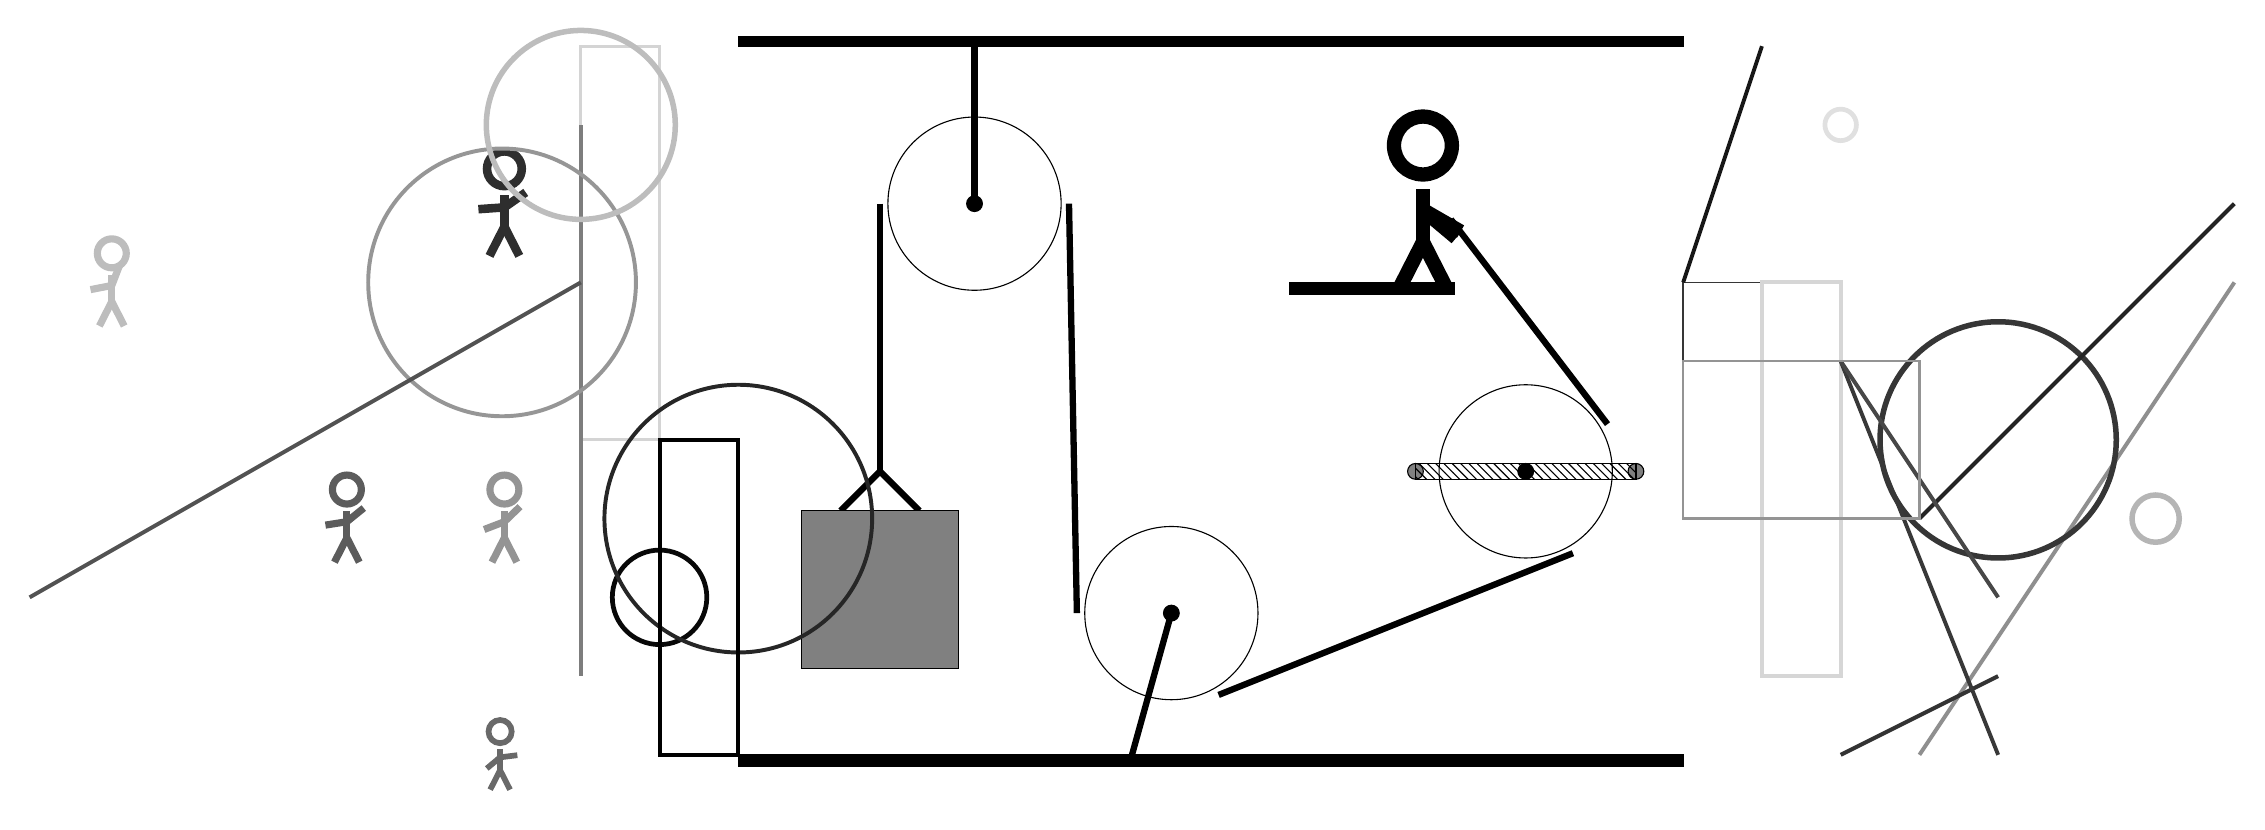
\begin{tikzpicture}
			%%%%% START %%%%%
			
			\draw[fill=black] (-2, 9) rectangle (10, 9.125);
			
			\draw (1, 7) circle (1.1);
			\draw[fill=black] (1, 7) circle (0.1);
			\draw[line width=0.8mm] (1, 9) -- (1, 7);
			
			\draw (3.5, 1.8) circle (1.1);
			\draw[fill=black] (3.5, 1.8) circle (0.1);
			\draw[line width=0.8mm] (3.5, 1.8) -- (3.0, 0);
			
			\draw[fill=white](8, 3.6) circle (1.1);
			\draw[fill=black] (8, 3.6) circle (0.1);
			\draw[fill=black!50] (9.4, 3.6) circle (0.1);
			\draw[fill=black!50] (6.6, 3.6) circle (0.1);
			\draw[pattern=north west lines, pattern color=black] (6.6, 3.7) rectangle (9.4, 3.5);
			
			\draw[line width=0.8mm](-0.7, 3.1) --  (-0.2, 3.6) -- (0.3, 3.1);
			\draw[fill=black!50] (-1.2, 3.1) rectangle (0.8, 1.1);
			
			\draw[line width=0.2mm, color=black!79] (11, 6) rectangle (10, 5);
			
			\draw [line width=0.6mm, color=black!97](-3, 2) circle (0.6);
			\draw[line width=0.4mm, color=black!17] (-4, 9) rectangle (-3, 4);
			\draw[line width=0.5mm, color=black!16] (11, 1) rectangle (12, 6);
			\draw[line width=0.5mm, color=black!44](13, 0) -- (17, 6);
			\draw[line width=0.5mm, color=black!91](10, 6) -- (11, 9);
			\node[line width=0.3mm, color=black!82] at (-5, 7) {\Strichmaxerl[6][4][35]};
			\draw [line width=0.5mm, color=black!85](-2, 3) circle (1.7);
			\draw[line width=0.5mm, color=black!51](-4, 8) -- (-4, 1);
			\draw[line width=0.5mm, color=black!80](12, 0) -- (14, 1);
			
			\draw [line width=0.6mm, color=black!12](12, 8) circle (0.2);
			\draw[line width=0.5mm, color=black!64](12, 5) -- (12, 5);
			\draw [line width=0.5mm, color=black!41](-5, 6) circle (1.7);
			\draw [line width=0.7mm, color=black!79](14, 4) circle (1.5);
			\draw[line width=0.5mm, color=black!78](12, 5) -- (14, 0);
			\node[line width=0.6mm, color=black!26] at (-10, 6) {\Strichmaxerl[5][11][69]};
			
			\draw[line width=0.5mm, color=black!86](13, 3) -- (17, 7);
			\draw[line width=0.5mm, color=black!68](-4, 6) -- (-11, 2);
			\node[line width=0.7mm, color=black!42] at (-5, 3) {\Strichmaxerl[5][21][44]};
			\draw [line width=0.7mm, color=black!29](16, 3) circle (0.3);
			\node[line width=0.7mm, color=black!59] at (-5, 0) {\Strichmaxerl[4][40][7]};
			\draw[line width=0.5mm, color=black!72](12, 5) -- (14, 2);
			\node[line width=0.7mm, color=black!64] at (-7, 3) {\Strichmaxerl[5][9][39]};
			\draw [line width=0.4mm, color=black!26](16, 4) circle (0.0);
			\draw[line width=0.5mm, color=black!100] (-3, 4) rectangle (-2, 0);
			
			\draw [line width=0.7mm, color=black!26](-4, 8) circle (1.2);
			\draw[line width=0.3mm, color=black!42] (10, 3) rectangle (13, 5);
			
			\draw[line width=0.8mm](-0.2, 7) -- (-0.2, 3.6);
			\centerarc[line width=0.8mm](1, 7)(180:0:1.2000000000000002)
			\draw[line width=0.8mm](2.2, 7) -- (2.3, 1.8);
			\centerarc[line width=0.8mm](3.5, 1.8)(180:300:1.2000000000000002);
			\draw[line width=0.8mm](4.1, 0.7608) -- (8.6, 2.5608);
			\centerarc[line width=0.8mm](8, 3.6)(300:390:1.2000000000000002);
			\draw[line width=0.8mm](9.0392, 4.2) -- (7.05, 6.8);
			
			\node at (6.75, 7) {\Strichmaxerl[10][-220][-30]};
			\draw[fill=black] (5, 6) rectangle (7.1, 5.85);
			
			\draw[fill=black] (-2, 0) rectangle (10, -0.15);
			
			%%%%% END %%%%%
		\end{tikzpicture}
	\end{figure}	
\end{document}